\documentclass{beamer}


\usepackage[french,english]{babel}

\usepackage[T1]{fontenc}

\usepackage[utf8]{inputenc}


\usetheme{Warsaw}
\title{Arêtes communes et utilisation}

\author{Clément Legrand}
\date{14 Juin 2018}

\begin{document}


\begin{frame}[plain]
\titlepage
\end{frame}

\section{Stochastisation}

\begin{frame}{Stochastisation \& results}
\begin{block}{Aléatoire}
Ajout d'aléatoire dans l'opérateur CE: calcul des échanges possibles, puis choix aléatoire.
\end{block}

\centering
\begin{tabular}{|c||c||c||c||c|c|}
   \hline
   ($\lambda;\mu;\nu$) & Best known & CW & Determinist & Mean & Best \\
   \hline
   0.1;1.3;1.8 & 949 & 1493 & 952 & 1041 & 989 \\
   \hline
   1.0;0.2;0.6 & 949 & 968 & 968 & 968 & 963 \\
   \hline
   0.0;1.1;1.4 & 949 & 1658 & 1037 & 1026 & 984 \\
   \hline
\end{tabular}

\end{frame}

\section{Utilisation des arêtes conservées}
\begin{frame}{Que faire des arêtes conservées ?}
On suppose que l'on a obtenu ces arêtes.
\begin{exampleblock}{Idées}
\begin{itemize}
\item On décide de ne plus y toucher lors des opérations locales.
\item On détruit les arêtes que l'on ne conserve pas, puis on reconstruit une nouvelle solution en se basant sur les arêtes conservées.
\end{itemize}
\end{exampleblock}

\end{frame}

\subsection{Conservation}

\begin{frame}{Algorithme conservant les arêtes}
\begin{block}{Description}
Arêtes à conserver définies après le calcul de la solution initiale.

Désormais, chaque opérateur vérifie qu'il ne modifie pas les arêtes qui doivent être conservées.
\end{block}

\begin{exampleblock}{Amélioration}
Changement des arêtes à conserver après chaque nouvelle amélioration ou si pas d'améliorations
\end{exampleblock}

\end{frame}

\begin{frame}{Résultats}
Les arêtes conservées sont choisies aléatoirement

Cas où les arêtes fixées sont non modifiables

\begin{tabular}{|c|c|c|c|c|c|}
   \hline
   ($\lambda;\mu;\nu$) & CW & Mean(Det) & Best(Det) & Mean(Sto) & Best(Sto) \\
   \hline
   0.8;0.0;1.0 & 981 & 976 & 970 & 977 & 957 \\
   \hline
   1.0;0.0;0.7 & 1016 & 1004 & 986 & 1001 & 973\\
   \hline
   0.6;1.8;0.9 & 1532 & 1169 & 1078 & 1084 & 1014\\
   \hline
   1.0;0.2;0.6 & 968 & 966 & 957 & 965 & 957 \\
   \hline
\end{tabular}

Cas où les fixées sont changées après chaque nouvelle amélioration, et s'il n'y a pas eu d'améliorations depuis quelques tours.
\begin{tabular}{|c|c|c|c|c|c|}
   \hline
   ($\lambda;\mu;\nu$) & CW & Mean(Det) & Best(Det) & Mean(Sto) & Best(Sto) \\
   \hline
   0.8;0.0;1.0 & 981 & 965 & 957 & 974 & 957 \\
   \hline
   1.0;0.0;0.7 & 1016 & 1000 & 983 & 998 & 960\\
   \hline
   0.6;1.8;0.9 & 1532 & 1044 & 972 & 1006 & 970\\
   \hline
   1.0;0.2;0.6 & 968 & 958 & 957 & 963 & 957 \\
   \hline
\end{tabular}
\end{frame}

\begin{frame}
\begin{exampleblock}{Conclusion}
Il est plus intéressant de changer les arêtes conservées au cours de l'algo.
\end{exampleblock}
\end{frame}



\subsection{Destruction}

\begin{frame}{Algorithme détruisant puis reconstruisant une solution}
\begin{block}{Description}
\begin{itemize}
\item Calcul SI
\item Choix des arêtes à conserver;
\item Suppression de toutes les arêtes non conservées;
\item Rattacher toutes les tournées isolées au dépôt;
\item Appliquer de nouveau CW;
\item Application de l'heuristique habituelle.
\end{itemize}
\end{block}

\end{frame}

\begin{frame}{Exemple}
Choix des arêtes communes entre SI et Best (arêtes vertes):
\begin{center}
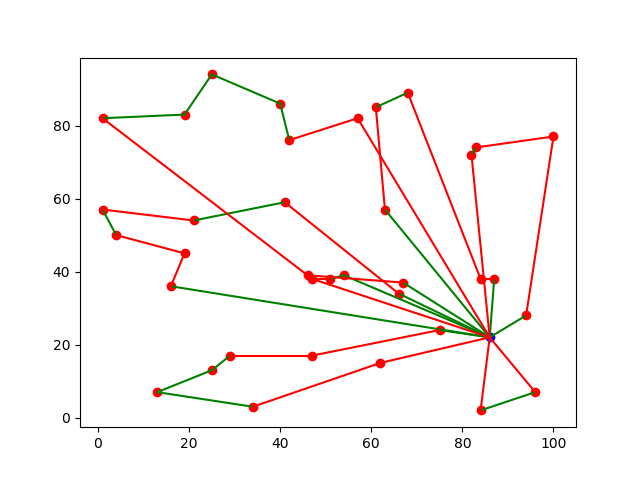
\includegraphics[scale=0.25]{edges_init.png}
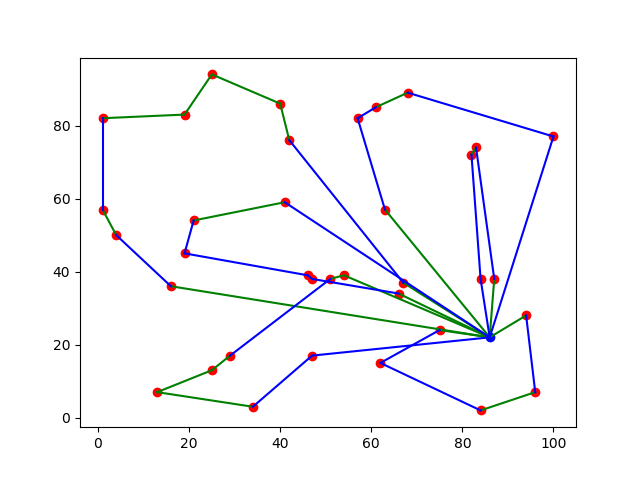
\includegraphics[scale=0.25]{edges_best.png}
\end{center}

Suppression et rattachement au dépôt:
\begin{center}
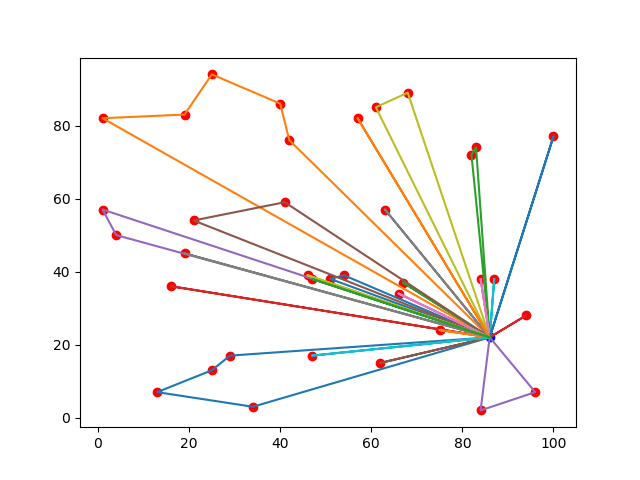
\includegraphics[scale=0.25]{reconstruction.png}
\end{center}
\end{frame}

\begin{frame}
Application de CW sur la solution:
\begin{center}
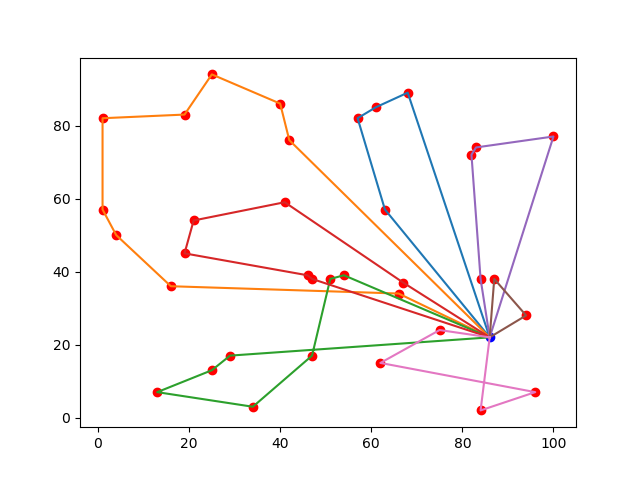
\includegraphics[scale=0.25]{new_solution.png}
\end{center}

Application de l'heuristique:
\begin{center}
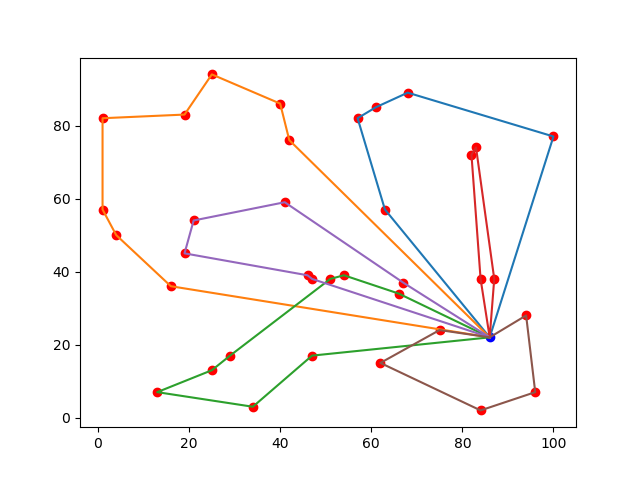
\includegraphics[scale=0.25]{best_solution.png}
\end{center}
\end{frame}

\section{Comment choisir les arêtes conservées ?}

\begin{frame}{Choix des arêtes conservées}
Plusieurs solutions pour choisir les arêtes à conserver:
\begin{itemize}
\item Utilisation des arêtes en commun entre SI et Best
\item Choix aléatoire d'arêtes
\end{itemize}
\end{frame}

\subsection{Utilisation de la meilleure solution}
\begin{frame}{Arêtes de la meilleure solution}
\begin{block}{Intérêt}
Permet de savoir si prendre les arêtes communes à la SI et à la best vont avoir un intérêt.
\end{block}
\begin{alertblock}{Problème}
On ne connaît pas forcément la meilleure solution au problème. 
\end{alertblock}
\end{frame}

\begin{frame}{Résultats}
Résultats observés sur quelques instances pour les heuristiques n'ayant pas d'aléatoire dans CE.
\begin{tabular}{|c|c|c|c|c|}
   \hline
   ($\lambda;\mu;\nu$) & CW & Det-classic & Det-cons & Det-dest \\
   \hline
   0.8;0.0;1.0 & 981 & 970 & 961 $|$ 957 & 954 \\
   \hline
   1.0;0.0;0.7 & 1016 & 992 & 998 $|$ 977 & 962 \\
   \hline
   0.6;1.8;0.9 & 1532 & 1034 & 1078 $|$ 957 & 977\\
   \hline
   1.0;0.2;0.6 & 968 & 968 & 957 $|$ 957 & 955 \\
   \hline
\end{tabular}

Idem pour les heuristiques ayant de l'aléatoire dans CE.
\begin{tabular}{|c|c|c|c|c|}
   \hline
   ($\lambda;\mu;\nu$) & CW & Sto-classic & Sto-cons & Sto-dest \\
   \hline
   0.8;0.0;1.0 &981 & 980 $|$ 973 & 972 $|$ 957 & 963 $|$ 960 \\
   \hline
   1.0;0.0;0.7 &1016& 1001 $|$ 973 & 993 $|$ 952 & 987 $|$ 965 \\
   \hline
   0.6;1.8;0.9 &1532& 1033 $|$ 990 & 1028 $|$ 963 & 1010 $|$ 973\\
   \hline
   1.0;0.2;0.6 &968& 968 $|$ 968 & 965 $|$ 957 & 988 $|$ 988 \\
   \hline
\end{tabular}
\end{frame}


\subsection{Choix aléatoire d'arêtes}

\begin{frame}{Arêtes aléatoires}

\begin{block}{Intérêt}
Toujours possible de les calculer
\end{block}

\begin{alertblock}{Problème}
Peu de contrôle sur les résultats
\end{alertblock}


\underline{Remarque}: pour les algorithmes "cons" on conserve $\frac{n}{10}$ arêtes, pour les algorithmes "dest" on en conserve $\frac{n}{2}$.

\end{frame}

\begin{frame}{Résultats}

\begin{tabular}{|c|c|c|c|c|}
   \hline
   ($\lambda;\mu;\nu$) & CW & Det-classic & Det-cons & Det-dest \\
   \hline
   0.8;0.0;1.0 &981 & 970 & 962 $|$ 957 & 1019 $|$ 957 \\
   \hline
   1.0;0.0;0.7 &1016& 992 & 1001 $|$ 975 & 1018 $|$ 963 \\
   \hline
   0.6;1.8;0.9 &1532& 1034& 1063 $|$ 963 & 1005 $|$ 957\\
   \hline
   1.0;0.2;0.6 &968& 968 & 958 $|$ 957 & 1016 $|$ 957 \\
   \hline
\end{tabular}

\begin{tabular}{|c|c|c|c|c|}
   \hline
   ($\lambda;\mu;\nu$) & CW & Sto-classic & Sto-cons & Sto-dest \\
   \hline
   0.8;0.0;1.0 &981 & 970 & 975 $|$ 957 & 1042 $|$ 986 \\
   \hline
   1.0;0.0;0.7 &1016& 992 & 997 $|$ 952 & 1072 $|$ 978 \\
   \hline
   0.6;1.8;0.9 &1532& 1034& 1021 $|$ 971 & 1008 $|$ 952\\
   \hline
   1.0;0.2;0.6 &968& 968 & 962 $|$ 957 & 1020 $|$ 970 \\
   \hline
\end{tabular}
\end{frame}

\begin{frame}{Conclusion}
\begin{itemize}
\item Nouvel algo en préparation
\item Etude de l'algo Det-dest
\end{itemize}
\end{frame}
\end{document}